\documentclass[10pt, compress, aspectratio=169]{beamer}

\usetheme{metropolis}

\usepackage{booktabs}
\usepackage[scale=2]{ccicons}

\usepackage{amsmath}
\usepackage{graphicx}


%Icons
\usepackage{fontawesome}

%Syntax highlight
\usepackage{listings,xcolor}
\usepackage{inconsolata}

\definecolor{dkgreen}{rgb}{0,.6,0}
\definecolor{dkblue}{rgb}{0,0,.6}
\definecolor{dkyellow}{cmyk}{0,0,.8,.3}

% Language: PHP
\lstset{
  language        = php,
  basicstyle      = \small\ttfamily,
  keywordstyle    = \color{dkblue},
  stringstyle     = \color{red},
  identifierstyle = \color{dkgreen},
  commentstyle    = \color{gray},
  emph            =[1]{php},
  emphstyle       =[1]\color{black},
  emph            =[2]{if,and,or,else},
  emphstyle       =[2]\color{dkyellow}
}

%\usepgfplotslibrary{dateplot}


\title{Using SMT solvers for binary analysis and exploitation}	
\subtitle{A primer on SMT, SMT solvers, Z3 \& angr}
\date{\today}
\author{Carl Svensson}
\institute{Nixucon 2018}

\begin{document}

\maketitle

\begin{frame}{About me}
  
	\begin{columns}
		\begin{column}{0.5\textwidth}  
  
  		\begin{itemize}
		  \item Carl Svensson, 27
		  \item MSc in Computer Science, KTH
		  \item Head of Security, KRY/LIVI
		  \item CTF-player, HackingForSoju
		  \item \faEnvelope \hskip 2mm calle.svensson@zeta-two.com
		  \item \faTwitter \hskip 2mm  @zetatwo
		  \item \faGlobe \hskip 2mm https://zeta-two.com
		\end{itemize}
		
		\end{column}
		\begin{column}{0.5\textwidth} 
			\begin{center}
			\includegraphics[width=0.4\textwidth]{images/kth.jpg}
			\end{center}
			\vspace{1cm}
			\includegraphics[width=\textwidth]{images/kry_logo.png}
		\end{column}
	\end{columns}
  
\end{frame}

\begin{frame}{Reverse engineering in 15 seconds?}

 \begin{itemize}
  \item Take stuff, e.g. software, apart
  \item Understand how it works
  \item Many possible goals
  \begin{itemize}
  	\item How can I reach a specific state?
  \end{itemize}  
  \end{itemize}    

\end{frame}


\begin{frame}{What is SMT?}

  \begin{itemize}
  \item Satisfiability modulo theories, SMT
  \item A bunch of variables
  \item A bunch of theories
  \begin{itemize}
    \item Theory = A bunch of rules
  \end{itemize}  
  \item A bunch of formulas
  \item Can we find values for all values s.t. all formulas are satisifed?
  \end{itemize}   

\end{frame}



\begin{frame}{SMT: Example 1}

	\begin{columns}
		\begin{column}{0.5\textwidth}
			\huge{$ x+13=37 $}
		\end{column}
		\begin{column}{0.5\textwidth}
			\includegraphics[width=0.8\textwidth]{images/happy.png}
		\end{column}
	\end{columns}
 
\end{frame}

\begin{frame}{SMT: Example 2}

	\begin{columns}
		\begin{column}{0.6\textwidth}
			\huge{$ x+y+13=37-z $} \\
			\huge{$ x-2 \cdot y+10=10 \cdot z $} \\
			\huge{$ 4\cdot x-z+13=37+y $} \\
		\end{column}
		\begin{column}{0.4\textwidth}
			\includegraphics[width=0.8\textwidth]{images/thinking.png}
		\end{column}
	\end{columns} 
	
\end{frame}

\begin{frame}{SMT: Example 3}

	\begin{columns}
		\begin{column}{0.7\textwidth}
			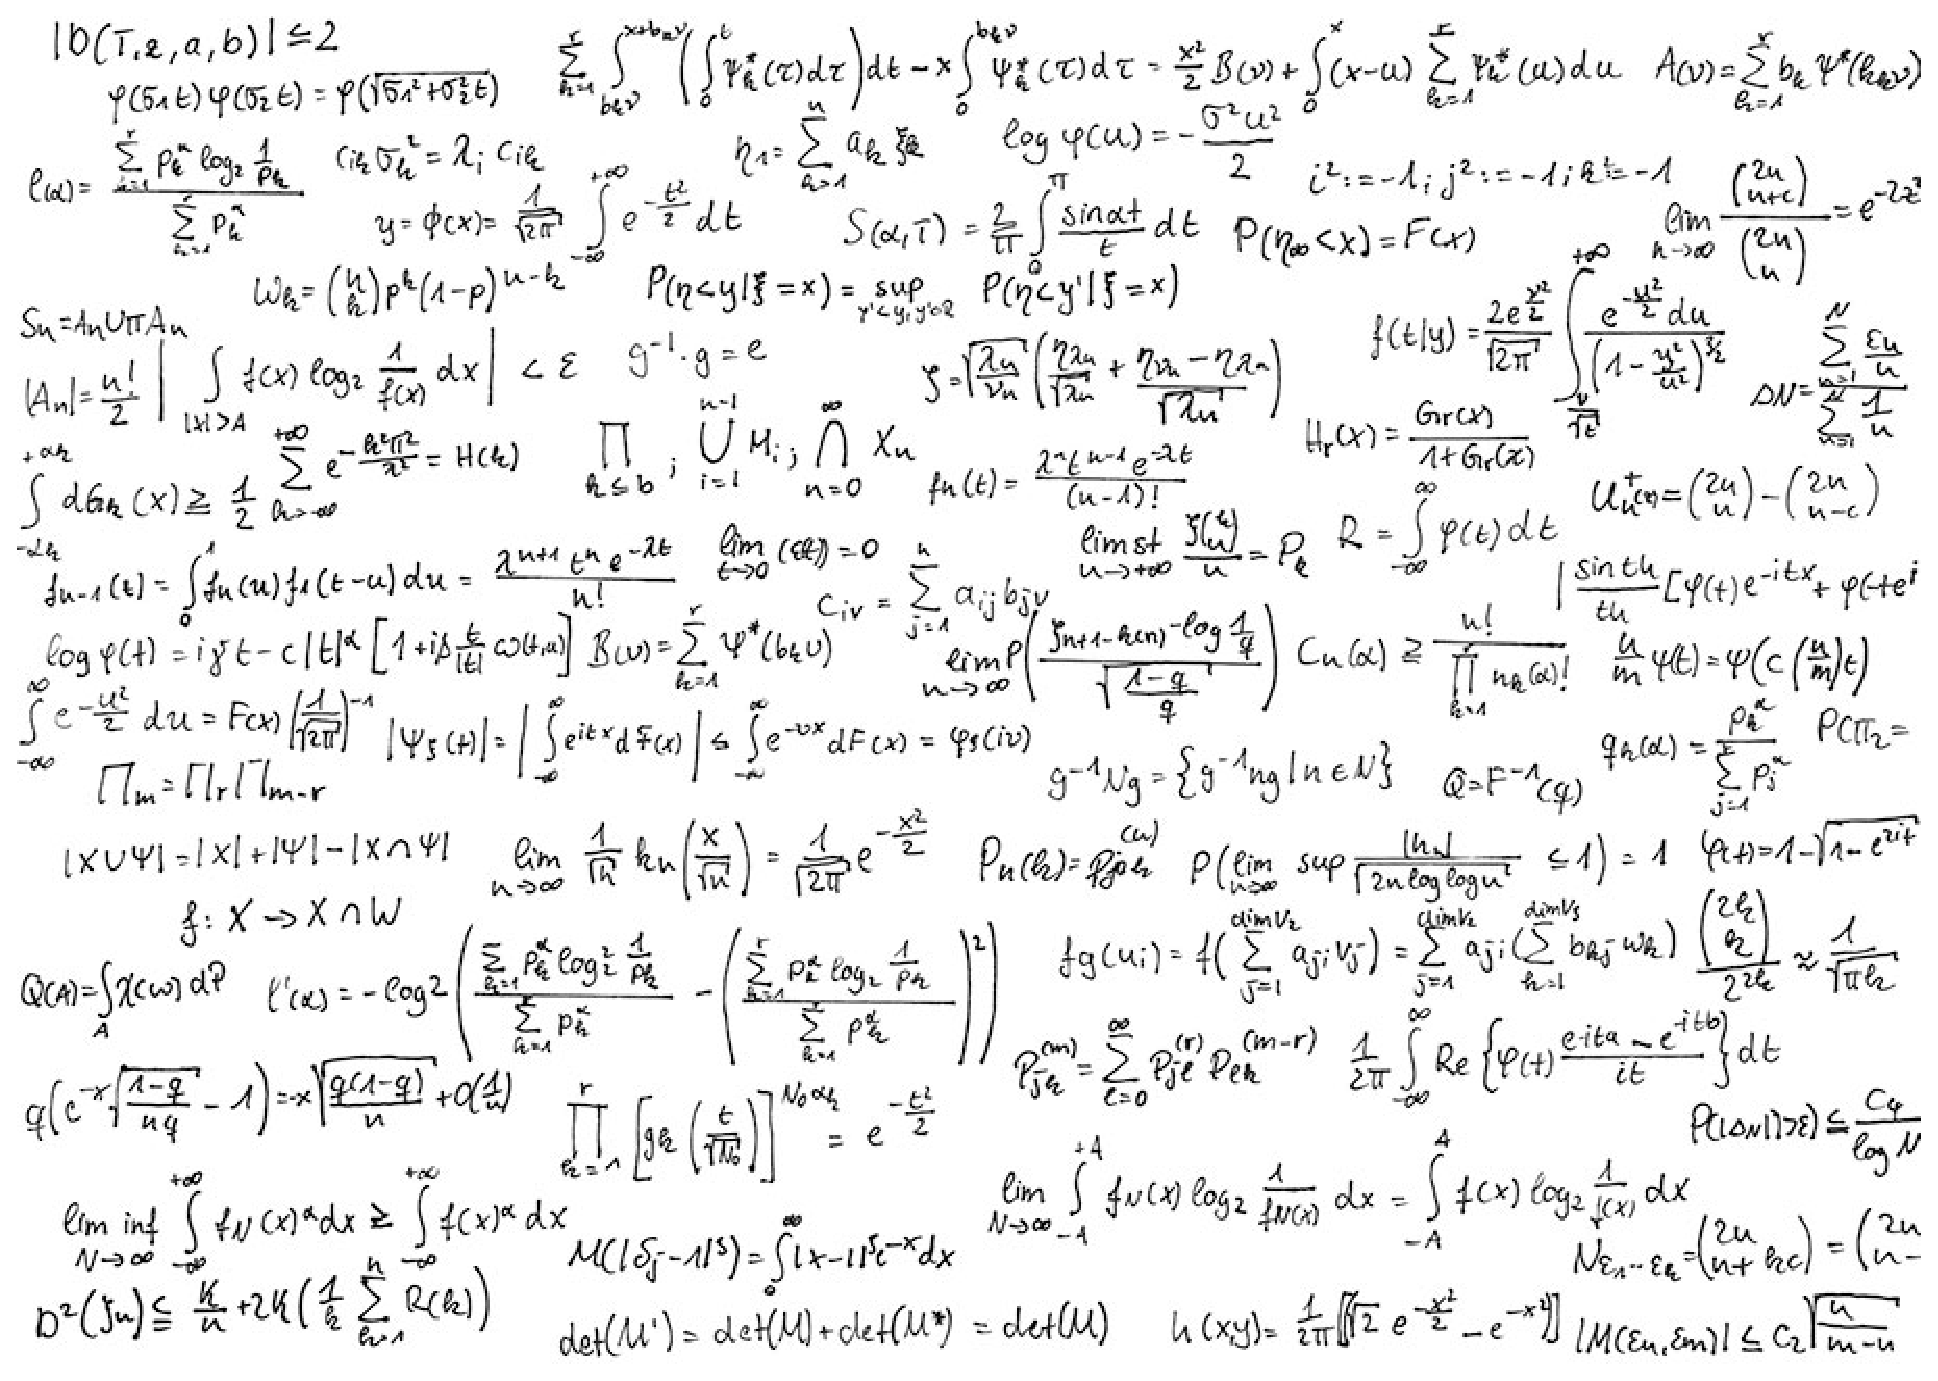
\includegraphics[width=\textwidth]{images/equations2.eps}
		\end{column}
		\begin{column}{0.3\textwidth}
			\includegraphics[width=0.8\textwidth]{images/angry.png}
		\end{column}
	\end{columns}  
	
\end{frame}


\begin{frame}{Microsoft to the rescue}

	\begin{columns}
		\begin{column}{0.6\textwidth}

		\begin{itemize}
		\item Can we automate? Yes!
		\item Microsoft Research
		\item Z3 Theorem Prover
		\begin{itemize}
			\item General purpose
			\item Own language
			\item Bindings for several languages
			\item Open source \& cross platform
		\end{itemize}   
		\end{itemize}   
		
		\end{column}
		\begin{column}{0.4\textwidth}
			\includegraphics{images/z3-logo.png}
		\end{column}
	\end{columns}		

\end{frame}

\begin{frame}{Using Z3 in Python}
  \includegraphics[width=0.4\textwidth]{images/z3-example.png}
\end{frame}


\begin{frame}{Using Z3 in RE}
\section{Throwback Thursday: Starcraft}
\end{frame}

\begin{frame}{Throwback Thursday: Starcraft}


	\begin{columns}
		\begin{column}{0.5\textwidth}
			\begin{itemize}
			\item Commercial software
			\item Released in 1998
			\begin{itemize}
				\item Simple protections
				\item Good starting point
			\end{itemize}
			\item Requires a serial key
			\item Can we create our own?
		\end{itemize}
		\end{column}
		\begin{column}{0.5\textwidth}
			\includegraphics[width=\textwidth]{images/starcraft.jpg}
		\end{column}
	\end{columns}

	
\end{frame}

\begin{frame}{Getting to the core: Installer}
	\includegraphics[width=0.7\textwidth]{images/sc1-1-setup.png}
\end{frame}

\begin{frame}{Getting to the core: Serial key input}
	\includegraphics[width=0.8\textwidth]{images/sc1-2-input-key.png}
\end{frame}

\begin{frame}{Getting to the core: Resource strings}
	\includegraphics[width=0.95\textwidth]{images/sc1-3-resources-strings.png}
\end{frame}

\begin{frame}{Getting to the core: Decompilation}
	\includegraphics[width=0.9\textwidth]{images/sc1-4-validator-rev-zoom.png}
\end{frame}

\begin{frame}{Getting to the core: Call graph}
	\includegraphics[width=0.9\textwidth]{images/sc1-5a-validator-graph.png}
\end{frame}

\begin{frame}{Getting to the core: Call graph}
	\includegraphics[width=0.9\textwidth]{images/sc1-5b-validator-graph.png}
\end{frame}

\begin{frame}{Getting to the core: Decompilation}
	\includegraphics[width=0.9\textwidth]{images/sc1-4-validator-rev-zoom.png}
\end{frame}

\begin{frame}{Z3: Formulating formulas}
	\includegraphics[width=0.7\textwidth]{images/sc1-6-z3-1.png}
\end{frame}

\begin{frame}{Z3: Formulating formulas}
	\includegraphics[width=0.7\textwidth]{images/sc1-6-z3-2.png}
\end{frame}

\begin{frame}{Symbolic execution}
  \begin{itemize}
    \item Symbols vs. concrete values
    \item Pro: Explore "all" paths
    \item Con: Exponential complexity
  \end{itemize}
\end{frame}

\begin{frame}{Once again, with fee... angr}

	\begin{columns}
		\begin{column}{0.6\textwidth}
	
		\begin{itemize}
		\item "python framework for analyzing binaries"
		\item "both static and dynamic symbolic (concolic)"
		\item Computer Security Lab at UC Santa Barbara
		\item Uses Z3 internally
		\end{itemize}
	\end{column}
		\begin{column}{0.4\textwidth}
			\includegraphics[width=\textwidth]{images/angr-logo.png}
		\end{column}
	\end{columns}	

\end{frame}

\begin{frame}{Angr management: Extracting the code}
	\includegraphics[width=0.9\textwidth]{images/sc1-7-validator-split.png}
\end{frame}

\begin{frame}{Angr management: Minimizing the code}
	\includegraphics[width=0.9\textwidth]{images/sc1-8-validator-clean-split.png}
\end{frame}

\begin{frame}{Angr management: Writing the explorer}
	\includegraphics[width=0.85\textwidth]{images/sc1-9-angr.png}
\end{frame}


\begin{frame}{Can we use even less effort?}

	\begin{columns}
		\begin{column}{0.6\textwidth}
	
		\begin{itemize}
		\item Extracting code is cumbersome
		\item Can't we use the code in place?
		\item "Call" directly into validator
		\item Symbolic argument
		\item Patch away irrelevant parts
		\end{itemize}
	\end{column}
		\begin{column}{0.4\textwidth}
			\includegraphics[width=\textwidth]{images/angr-logo.png}
		\end{column}
	\end{columns}	

\end{frame}

\begin{frame}{Full fury: Writing the explorer}
  \includegraphics[width=0.4\textwidth]{images/sc1-10-angr2-c.png}
\end{frame}

\begin{frame}{Full fury: Writing the explorer}
  \includegraphics[width=\textwidth]{images/sc1-10-angr2-a.png}
\end{frame}

\begin{frame}{Full fury: Writing the explorer}
  \includegraphics[width=\textwidth]{images/sc1-10-angr2-b.png}
\end{frame}

\begin{frame}{Using Z3 in RE}
\section{What about exploitation?}
\end{frame}


\begin{frame}{Exploitation}
  \begin{itemize}
    \item IP control
    \item Satisfy condition
  \end{itemize}
\end{frame}

\begin{frame}{Exploitation with angr}
  \begin{itemize}
    \item Find execution path
    \item Constrain execution
    \item Satisfy condition
  \end{itemize}
\end{frame}

\begin{frame}{Example from Security Fest CTF}
  \begin{itemize}
    \item Function pointer lookup
    \item Index OOB
    \item Hook messy function
  \end{itemize}
\end{frame}

\begin{frame}{angr exploitation example}
  \includegraphics[width=0.8\textwidth]{images/exploit-2-ida.png}
\end{frame}

\begin{frame}{angr exploitation example}
  \includegraphics[width=\textwidth]{images/exploit-1-angr-a.png}
\end{frame}

\begin{frame}{angr exploitation example}
  \includegraphics[width=0.5\textwidth]{images/exploit-2-ida2.png}
\end{frame}

\begin{frame}{angr exploitation example}
  \includegraphics[width=\textwidth]{images/exploit-1-angr-b.png}
\end{frame}

\begin{frame}[fragile]{angr exploitation example}

\begin{lstlisting}[language=bash]
> python exploit_angr.py
Choice: 2147483648
RDX: fffffffffffffffe
\end{lstlisting}

\begin{lstlisting}[language=bash]
> ./bowrain_581bbadaafd23051a25ccb4adc80b670
...
: 2147483648
[1] 17059 segmentation fault (core dumped)
\end{lstlisting}

\end{frame}


\begin{frame}{Using Z3 in RE}
\section{Even deobfuscation?!}
\end{frame}

\begin{frame}{Obfuscation}
  \begin{itemize}
    \item Make code hard to read
    \begin{itemize}
      \item for humans
      \item for computers
    \end{itemize}
    \item Control flow flattening
    \item Packer
    \item Dropper
    \item VM
    \item Dead code
  \end{itemize}
\end{frame}

\begin{frame}{Deobfuscation in general}
  \begin{itemize}
    \item Undo the mess
    \item Hard problem
  \end{itemize}
\end{frame}

\begin{frame}{Deobfuscation of dead code with angr}
  \begin{itemize}
    \item Prove that dead code is dead
    \item Prove uniqueness of value
  \end{itemize}
\end{frame}

\begin{frame}{Example: indirect jmp deobfuscator}
\begin{center}
  \includegraphics[width=0.6\textwidth]{images/deobf-1-ida1.png}
 \end{center}
\end{frame}

\begin{frame}{Example from mobile app}
  \begin{itemize}
    \item Find "jmp reg"
    \item Search callgraph backwards
    \item Search forward
    \item Simplify expression
    \item Replace code
  \end{itemize}
\end{frame}

\begin{frame}{Example: indirect jmp deobfuscator}
\begin{center}
  \includegraphics[width=0.8\textwidth]{images/deobf-4-angr1.png}
 \end{center}
\end{frame}

\begin{frame}{Example: indirect jmp deobfuscator}
\begin{center}
  \includegraphics[width=0.8\textwidth]{images/deobf-5-angr2.png}
 \end{center}
\end{frame}


\begin{frame}{Example: indirect jmp deobfuscator}
\begin{center}
  \includegraphics[width=0.5\textwidth]{images/deobf-2-ida2.png}
   \end{center}
\end{frame}

\begin{frame}{Example: indirect jmp deobfuscator}
\begin{center}
  \includegraphics[width=0.5\textwidth]{images/deobf-3-ida3.png}
   \end{center}
\end{frame}

\begin{frame}[standout]
Thanks for listening!
\end{frame}


\end{document}
